\documentclass[12pt]{article}
\usepackage[utf8]{inputenc}
\usepackage[T1]{fontenc}
\usepackage[spanish]{babel}
\usepackage{listings}
\usepackage{xcolor}
\usepackage{geometry}
\usepackage{enumitem}
\usepackage{parskip} 
\usepackage{microtype}
\usepackage{graphicx}
\usepackage{xcolor}

\definecolor{codebg}{RGB}{248,248,248}
\definecolor{codeframe}{RGB}{220,220,220}
\definecolor{codekeyword}{RGB}{0,102,204}
\definecolor{codecomment}{RGB}{0,153,0}
\definecolor{codestring}{RGB}{163,21,21}
\definecolor{codenumbers}{gray}{0.5}
\geometry{a4paper, margin=2.5cm}

\title{Trabajo 1\\ Paradigmas de la Programaci\'on}
\author{Rapha\"el Maufroy \& Jos\'e Salazar Cabello}
\date{Abril 2025}

\lstdefinestyle{customc}{
  language=C++,
  backgroundcolor=\color{codebg},
  frame=single,
  rulecolor=\color{codeframe},
  keywordstyle=\color{codekeyword}\bfseries,
  commentstyle=\color{codecomment}\itshape,
  stringstyle=\color{codestring},
  basicstyle=\ttfamily\footnotesize,
  numbers=left,
  numberstyle=\tiny\color{codenumbers},
  stepnumber=1,
  numbersep=10pt,
  breaklines=true,
  showstringspaces=false,
  tabsize=2,
  literate={á}{{\'a}}1 {é}{{\'e}}1 {í}{{\'i}}1 {ó}{{\'o}}1 {ú}{{\'u}}1
           {Á}{{\'A}}1 {É}{{\'E}}1 {Í}{{\'I}}1 {Ó}{{\'O}}1 {Ú}{{\'U}}1
           {ñ}{{\~n}}1 {Ñ}{{\~N}}1
}

\begin{document}

\begin{titlepage}
    \centering
    \vspace*{2cm}
    {\scshape\LARGE Universidad Andr\'es Bello \par}
    \vspace{1cm}
    {\scshape\Large Facultad de Ingenier\'ia\par}
    \vspace{1.5cm}
    {\Large Paradigmas de la Programaci\'on\par}
    \vspace{0.5cm}
    {\huge\bfseries Trabajo 1\\La taxonom\'ia de Bloom \par}
    \vspace{2cm}
    {\Large Autores: \\Rapha\"el Maufroy\\Jos\'e Salazar Cabello\par}
    \vspace{0.5cm}
    {\Large Profesor: Juan Calder\'on Maureira\par}
    \vspace{0.5cm}
    {\Large Fecha: Abril 2025\par}
    \vfill
    {\large A\~no Acad\'emico: 2025, Semestre 1\par}
\end{titlepage}

\newpage
\subsection{Diagrama de Clases}

A continuación, se presenta el diagrama de clases correspondiente a la solución planteada. Este diagrama permite visualizar de manera general las relaciones entre las distintas clases desarrolladas, sus atributos principales y los métodos más relevantes que posee cada una.
\vspace{0.5cm}
\begin{figure}[h!]
    \centering
    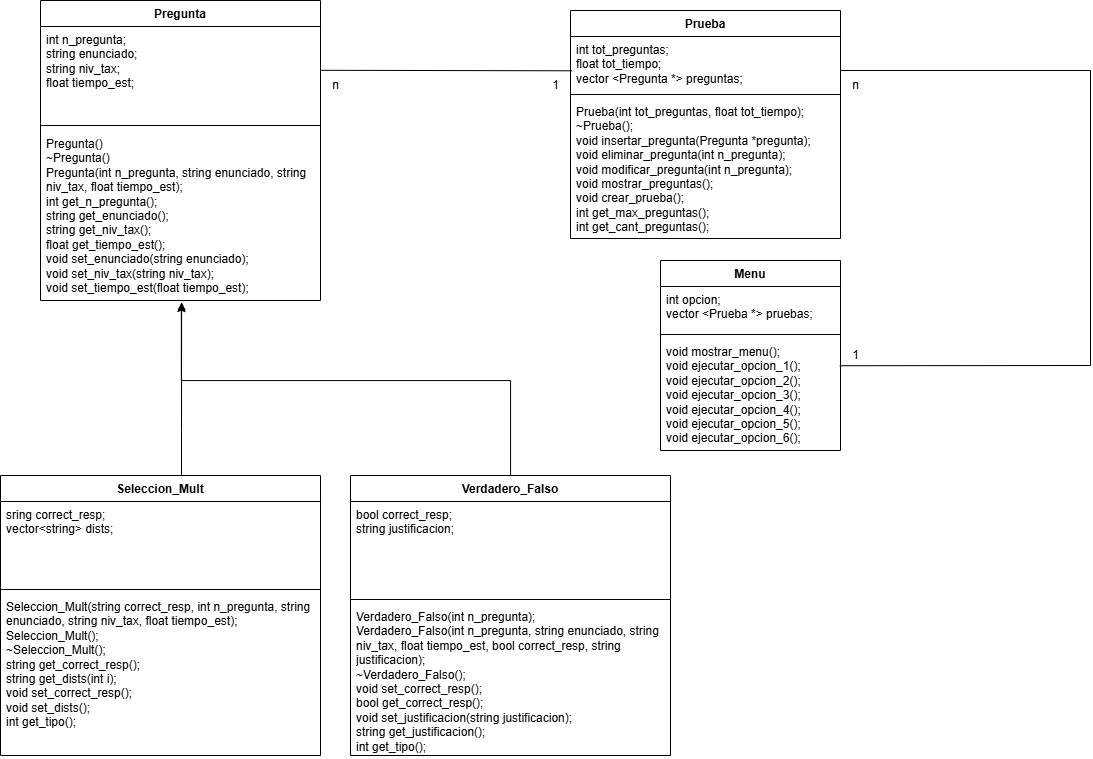
\includegraphics[width=1\linewidth]{TAREA_1PARAPROGRA.png}
    \caption{Diagrama de clases del sistema desarrollado.}
    \label{fig:diagrama-clases}
\end{figure}
\newpage

\section{Introducci\'on}
El presente trabajo tiene como objetivo desarrollar un sistema en C++ que permita a un usuario crear y gestionar pruebas escritas utilizando la Taxonom\'ia de Bloom como referencia principal.

Dentro del desarrollo del trabajo se busc\'o aplicar conceptos fundamentales de programaci\'on orientada a objetos, como lo son la herencia, el polimorfismo y el manejo de memoria din\'amica. Adem\'as, se consider\'o dise\~nar una soluci\'on modular y estructurada que permita un f\'acil mantenimiento y comprensi\'on del c\'odigo.

La funcionalidad central del sistema consiste en gestionar pruebas compuestas por distintos tipos de preguntas, tales como preguntas de Verdadero o Falso y preguntas de Selecci\'on M\'ultiple. Cada una de estas preguntas se encuentra asociada a un nivel taxon\'omico, lo que permite categorizar y evaluar las habilidades que se desean medir en el evaluado.

En este informe se presentar\'a:
\begin{itemize}
    \item La descripci\'on detallada de la soluci\'on implementada
    \item Las decisiones de dise\~no tomadas en el desarrollo
    \item La estructura y funcionamiento del sistema
    \item Las conclusiones y reflexiones sobre el trabajo realizado
\end{itemize}

\section{Descripci\'on de la soluci\'on}
La soluci\'on se estructura en cuatro clases principales:

\subsection{Clase Pregunta}
La clase base \texttt{Pregunta} define la estructura com\'un para todos los tipos de preguntas:

\begin{lstlisting}[style=customc]
class Pregunta {
  private:
    int n_pregunta;
    string enunciado;
    string niv_tax;
    float tiempo_est;
  public:
    Pregunta(int n_pregunta, string enunciado, string niv_tax, float tiempo_est);
    virtual ~Pregunta();
    // Métodos getters y setters
    virtual void set_correct_resp()=0;
    virtual int get_tipo();
    void set_tiempo_est(float tiempo_est);
    float get_tiempo_est();
};
\end{lstlisting}

Los atributos principales incluyen:
\begin{itemize}
    \item \texttt{n\_pregunta}: Identificador \'unico de la pregunta
    \item \texttt{enunciado}: Texto de la pregunta
    \item \texttt{niv\_tax}: Nivel taxon\'omico seg\'un Bloom
    \item \texttt{tiempo\_est}: Tiempo estimado para responder
\end{itemize}

\subsection{Clases Derivadas}

\subsubsection{Clase Seleccion\_Mult}
Esta clase implementa las preguntas de selecci\'on m\'ultiple:

\begin{lstlisting}[style=customc]
class Seleccion_Mult : public Pregunta {  
  private:
    string correct_resp;
    vector<string> dists;
  public:
    Seleccion_Mult(string correct_resp, int n_pregunta, 
                   string enunciado, string niv_tax, 
                   float tiempo_est);
    ~Seleccion_Mult();
    void set_correct_resp();
    void set_dists();
    string get_dists(int i);
    int get_tipo() { return 2; }
};
\end{lstlisting}

\subsubsection{Clase Verdadero\_Falso}
Esta clase maneja las preguntas de verdadero o falso:

\begin{lstlisting}[style=customc]
class Verdadero_Falso : public Pregunta {
  private:
    bool correct_resp;
    string justificacion;
  public:
    Verdadero_Falso(int n_pregunta, string enunciado, 
                    string niv_tax, float tiempo_est,
                    bool correct_resp, string justificacion);
    ~Verdadero_Falso();
    void set_correct_resp();
    bool get_correct_resp();
    void set_justificacion(string justificacion);
    string get_justificacion();
    int get_tipo() { return 1; }
};
\end{lstlisting}

\subsection{Clase Prueba}
La clase \texttt{Prueba} gestiona un conjunto de preguntas:

\begin{lstlisting}[style=customc]
class Prueba {
  private:
    int tot_preguntas;
    float tot_tiempo;
    vector<Pregunta *> preguntas;
    void recalcular_tiempo_total();
  public:
    Prueba(int tot_preguntas, float tot_tiempo);
    ~Prueba();
    void insertar_pregunta(Pregunta *pregunta);
    void eliminar_pregunta(int n_pregunta);
    void modificar_pregunta(int n_pregunta);
    void mostrar_preguntas();
    int get_max_preguntas();
    int get_cant_preguntas();
    float get_tiempo_total() const { return tot_tiempo; }
};
\end{lstlisting}

Un ejemplo de implementaci\'on de uno de sus m\'etodos principales es:

\begin{lstlisting}[style=customc]
void Prueba::modificar_pregunta(int n_pregunta) {
  int tipo = this->preguntas[n_pregunta - 1]->get_tipo();
  if (tipo == 1) {  // Verdadero_Falso
    string input;
    cout << "Modificar el tiempo estimado: "<< endl;
    cin.ignore();
    getline(cin,input);
    if(!input.empty()){
        this->preguntas[n_pregunta - 1]->set_tiempo_est(stof(input));
        this->recalcular_tiempo_total();
    }
    // ... más código de modificación
  } else { // Seleccion_Mult
    // ... (obtener input para enunciado, nivel tax, tiempo)
    cout << "Modificar el tiempo estimado: "<< endl;
    cin.ignore();
    getline(cin,input);
    if(!input.empty()){
        this->preguntas[n_pregunta - 1]->set_tiempo_est(stof(input));
        this->recalcular_tiempo_total();
    }
    // ... más código de modificación
  }
}
\end{lstlisting}

La implementación del método \texttt{recalcular\_tiempo\_total()} asegura que el tiempo total se mantenga sincronizado con la suma de los tiempos individuales de cada pregunta:

\begin{lstlisting}[style=customc]
void Prueba::recalcular_tiempo_total() {
    float nuevo_tiempo = 0;
    for (Pregunta* pregunta : preguntas) {
        nuevo_tiempo += pregunta->get_tiempo_est();
    }
    this->tot_tiempo = nuevo_tiempo;
}
\end{lstlisting}

El sistema actualiza automáticamente el tiempo total en los siguientes casos:

\begin{itemize}
    \item Al insertar una nueva pregunta:
    \begin{lstlisting}[style=customc]
    void Prueba::insertar_pregunta(Pregunta *pregunta) {
        this->preguntas.push_back(pregunta);
        this->recalcular_tiempo_total();
    }
    \end{lstlisting}

    \item Al eliminar una pregunta existente:
    \begin{lstlisting}[style=customc]
    void Prueba::eliminar_pregunta(int n_pregunta) {
        this->preguntas.erase(this->preguntas.begin() + n_pregunta - 1);
        this->recalcular_tiempo_total();
    }
    \end{lstlisting}

    \item Al modificar el tiempo estimado de una pregunta:
    \begin{lstlisting}[style=customc]
    // En el método modificar_pregunta
    if(!input.empty()) {
        this->preguntas[n_pregunta - 1]->set_tiempo_est(stof(input));
        this->recalcular_tiempo_total();
    }
    \end{lstlisting}
\end{itemize}

Esta implementación ofrece varias ventajas:

\begin{itemize}
    \item \textbf{Consistencia}: El tiempo total siempre refleja la suma real de los tiempos de las preguntas
    \item \textbf{Automatización}: No requiere intervención manual para mantener el tiempo actualizado
    \item \textbf{Encapsulamiento}: El método \texttt{recalcular\_tiempo\_total()} es privado, asegurando que solo se llame cuando es necesario
    \item \textbf{Flexibilidad}: Permite modificar tiempos individuales manteniendo la coherencia del tiempo total
\end{itemize}

\subsection{Clase Menu}
La clase \texttt{Menu} implementa la interfaz de usuario y la l\'ogica principal del programa, definida en \texttt{utils.h} e implementada en \texttt{utils.cpp}. Esta clase es responsable de la interacci\'on con el usuario y la gesti\'on de las pruebas:

\begin{lstlisting}[style=customc]
class Menu {
  private:
    int opcion;
    vector<Prueba *> pruebas;
  public:
    void mostrar_menu();
    void ejecutar_opcion_1();  // Crear prueba
    void ejecutar_opcion_2();  // Insertar pregunta
    void ejecutar_opcion_3();  // Eliminar pregunta
    void ejecutar_opcion_4();  // Modificar pregunta
    void ejecutar_opcion_5();  // Mostrar preguntas
    void ejecutar_opcion_6();  // Eliminar prueba
};
\end{lstlisting}

La implementaci\'on del men\'u sigue un patr\'on de dise\~no modular, donde cada opci\'on est\'a encapsulada en su propio m\'etodo. Por ejemplo, la creaci\'on de una prueba:

\begin{lstlisting}[style=customc]
void Menu::ejecutar_opcion_1() {  
  int tot_preguntas;
  float tot_tiempo;
  string input;
  limpiar_pantalla();
  cout << "Crear prueba" << endl;
  
  do {
    cout << "Ingrese el numero de preguntas (debe ser positivo): ";
    getline(cin, input);
    try { tot_preguntas = stoi(input); } catch (...) { tot_preguntas = 0; }
  } while (tot_preguntas <= 0);

  do {
    cout << "Ingrese el tiempo total estimado (o 0 para usar el valor por defecto): ";
    getline(cin, input);
    try {
      tot_tiempo = stof(input);
      if (tot_tiempo < 0) tot_tiempo = 0;
    } catch (...) { tot_tiempo = 0; }
  } while (tot_tiempo < 0);

  if (tot_preguntas > 0) {
    if (tot_tiempo <= 0) {
      tot_tiempo = tot_preguntas * 3.0f; // Tiempo por defecto
      cout << "Usando tiempo por defecto: " << tot_tiempo << " minutos" << endl;
    }
    Prueba *prueba = new Prueba(tot_preguntas, tot_tiempo);
    this->pruebas.push_back(prueba);
    cout << "Prueba creada exitosamente." << endl;
  }  
}
\end{lstlisting}

Las principales decisiones de dise\~no en la clase Menu incluyen:

\begin{enumerate}
    \item \textbf{Gesti\'on de Memoria Din\'amica}: Utilizamos un vector de punteros a \texttt{Prueba} para mantener las pruebas creadas:
    \begin{lstlisting}[style=customc]
    vector<Prueba *> pruebas;
    
    // En ejecutar_opcion_6 (eliminar prueba):
    delete this->pruebas[id_prueba-1];
    this->pruebas.erase(this->pruebas.begin() + id_prueba - 1);
    \end{lstlisting}

    \item \textbf{Validaci\'on de Entradas}: Implementamos validaciones para asegurar la integridad de los datos:
    \begin{lstlisting}[style=customc]
    if (id_prueba > 0 && id_prueba <= this->pruebas.size()) {
      if (id_pregunta > 0 && 
          id_pregunta <= this->pruebas[id_prueba-1]->get_cant_preguntas()) {
        // Operación válida
      }
    }
    \end{lstlisting}

    \item \textbf{Interfaz de Usuario}: Dise\~namos una interfaz clara y amigable:
    \begin{itemize}
        \item Mensajes informativos para cada operaci\'on
        \item Limpieza de pantalla entre operaciones
        \item Pausas para mejor legibilidad (\texttt{this\_thread::sleep\_for})
    \end{itemize}

    \item \textbf{Modularidad}: Cada operaci\'on est\'a encapsulada en su propio m\'etodo, lo que facilita:
    \begin{itemize}
        \item Mantenimiento del c\'odigo
        \item Depuraci\'on de errores
        \item Extensibilidad del sistema
    \end{itemize}
\end{enumerate}

\subsection{Decisiones de Dise\~no}
Las principales decisiones de dise\~no tomadas incluyen:

\begin{enumerate}
    \item \textbf{Herencia y Polimorfismo}: Utilizamos una jerarqu\'ia de clases para manejar los diferentes tipos de preguntas. Por ejemplo, el m\'etodo virtual \texttt{get\_tipo()} nos permite identificar el tipo de pregunta sin necesidad de hacer casting:
    \begin{lstlisting}[style=customc]
    virtual int get_tipo();  // Implementado en clase base y derivadas
    int get_tipo() { return 1; } // En Verdadero_Falso
    int get_tipo() { return 2; } // En Seleccion_Mult
    \end{lstlisting}

    \item \textbf{Gesti\'on de Memoria Din\'amica}: Implementamos un sistema de gesti\'on de memoria usando punteros y vectores de la STL:
    \begin{lstlisting}[style=customc]
    vector<Pregunta *> preguntas;  // Vector de punteros
    ~Prueba() {
      for(auto p : preguntas) {
        delete p;  // Liberación de memoria
      }
    }
    \end{lstlisting}
\end{enumerate}

\section{Conclusi'on}
El desarrollo de este trabajo nos permiti'o implementar de manera pr'actica los principales conceptos de la programaci'on orientada a objetos en C++. Logramos crear un sistema modular y estructurado que gestiona eficientemente pruebas y preguntas siguiendo la taxonom'ia de Bloom.

El uso de herencia y polimorfismo result'o fundamental para manejar los diferentes tipos de preguntas de manera uniforme, mientras que el uso de memoria din'amica nos permiti'o una gesti'on flexible de las pruebas y sus componentes.

La soluci'on desarrollada demuestra la aplicabilidad de los conceptos de POO en problemas reales, resultando en un c'odigo mantenible, extensible y bien estructurado que cumple con todos los requerimientos establecidos.

\subsection{Cumplimiento de Objetivos}
Se alcanzaron satisfactoriamente los siguientes objetivos:
\begin{itemize}
    \item Implementaci'on de un sistema funcional para la gesti'on de pruebas
    \item Incorporaci'on efectiva de los niveles taxon'omicos de Bloom
    \item Desarrollo de una interfaz de usuario intuitiva
    \item Implementaci'on de todas las operaciones CRUD requeridas
\end{itemize}

\subsection{Reflexi'on sobre el Trabajo}
El desarrollo de este proyecto permiti'o:
\begin{itemize}
    \item Profundizar en la aplicaci\'on pr\'actica de conceptos de POO
    \item Comprender la importancia de un buen dise\~no de software
    \item Desarrollar habilidades en la gesti\'on de memoria din\'amica
    \item Implementar soluciones modulares y extensibles
\end{itemize}

\end{document} 